\chapter{模擬環境}
%\renewcommand{\baselinestretch}{10.0} %設定行距
\section{模擬模型}
 在模擬的模型上,延用了學長之前組建的實體3D列印機,並將其轉為虛擬模型後放入CoppeliaSim,進行組裝、配置後以simExtFIBR3D.dll擴充CoppeliaSim將其與GCodeInterpreter程式進行整合,用以達成使用GCode控制CoppeliaSim中的3D列印機進行模擬列印展示之功能。\\
\begin{figure}[hbt!]
\center
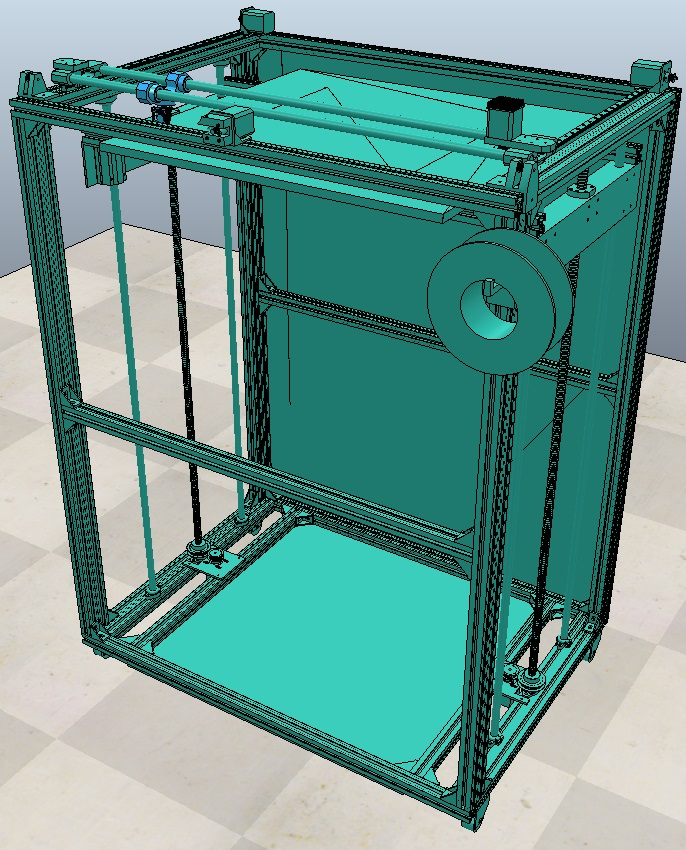
\includegraphics[width=13cm]{組合圖}
\caption{\Large 組合圖}
\label{組合圖}
\end{figure}

\newpage

\section{CoppeliaSim}
 CoppeliaSim是一套具有整合開發環境的機器人模擬軟體,基於分佈式控制體系架構,可以利用寫入嵌入式腳本、插件、ROS、BlueZero節點、RemoteAPI客戶端或自定義解決方案達成模型控制之效果。\\
\begin{figure}[hbt!]
\center

\includegraphics[width=10cm]{CoppeliaSim}
\caption{\Large CoppeliaSim Logo}
\end{figure}

並且在CoppeliaSim中,控制器可以用C / C ++、Python、Java、Lua、Matlab或Octave進行編寫。\\
\subsection{使用原因}
 本模擬之最終目標是希望可以在虛擬環境中進行3D列印的結果展示,通過虛擬環境中的模擬後,在每次修改零件並更新Gcode後可以直接展示列印的狀況,且在虛擬環境中不會有費用的支出,所以可以用於檢視所列印出之成果後,再進行圖檔修正或設計修改,除此之外CoppeliaSim的虛擬環境更接近真實環境,基於以上原因,所以此專題選擇CoppeliaSim做為模擬的環境。\\
\subsection{RemoteAPI}
 RemoteAPI(Remote Application Programming Interface)是CoppeliaSim API框架的一部分。它允許CoppeliaSim與外部應用程序之間的通訊,是跨平台並支持服務調用和雙向數據流。有兩個不同的版本/框架分別為:Remote API 和The B0-based remote API。\\
\subsection{功能列}
\begin{enumerate}
\item 以下為簡易功能說明:
\begin{figure}[hbt!]
\center
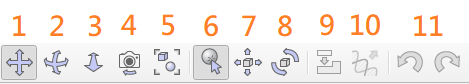
\includegraphics[width=11cm]{toolBar}
\caption{\Large CoppeliaSim 工具列}
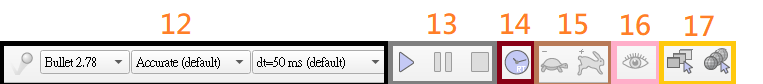
\includegraphics[width=13cm]{toolBar2}
\caption{\Large CoppeliaSim 工具列(續)}
\end{figure}
\begin{table}[hbt!]
\center
\large
\setlength{\tabcolsep}{0.75cm}{
\begin{tabular}{|c|c|c|c|}
\hline  代號 & 功能說明 & 代號 & 功能說明\\
\hline  1 &畫面平移& 10 &複製所有設定\\
\hline  2 &畫面旋轉& 11 &回復/取消回復\\
\hline  3 &畫面縮放&12&模擬設定\\
\hline  4 &畫面視角&13&開始/暫停/停止 模擬\\
\hline  5 &畫面縮放至適當大小&14&即時模擬切換\\
\hline  6 &選取物件&15&模擬速度控制\\
\hline  7 &移動物件&16&線程渲染/視覺化\\
\hline  8 &旋轉物件&17&場景/頁面 選擇\\
\hline  9 &加入/移出 樹狀結構&&\\
\hline
\end{tabular}}
\caption{\Large 功能說明}
\end{table}
\newpage
%\item 模擬執行\\%
\end{enumerate}
\section{FIBR3DEmul}
 FIBR3DEmul--是一個適用於3軸或3軸以上的FDM(熔融沉積成型)列印機,進行虛擬列印的開源軟體,在它之中包含了GCodeInterpreter(GCode解析器)、使用CMake生成的simExtFIBR3D.dll\\
\subsection{GCodeInterpreter}
\begin{figure}[hbt!]
\begin{center}
\includegraphics[width=14cm]{Gcode}
\caption{\Large GCodeInterpreter 介面功能介紹}\label{GCode}
\end{center}
\end{figure}
\newpage


\chapter{整體模擬流程}
\section{使用Inventor繪製uArm零件}
 模擬的第一步是先將設計後的uArm零件使用Inventor繪製出來後,再將其轉為Cura程式可接受的STL檔案格式。\\
\begin{figure}[hbt!]
\begin{center}
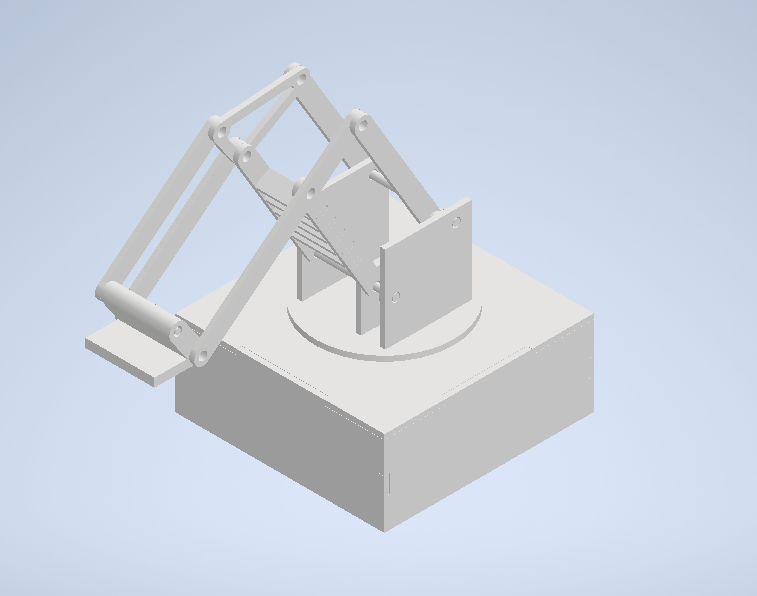
\includegraphics[width=8cm]{Inventor1}
\caption{\Large 使用Inventor繪製零件}\label{Inventor1}
\end{center}
\end{figure}
\section{使用Cura轉出G-Code檔}
 第二步將把上一步轉出的STL檔案轉入Cura程式中,可將零件們進行排列或旋轉方向放置到最佳的列印位置,進行切片後,轉出所需的G-Code檔案。\\
\begin{figure}[hbt!]
\begin{center}
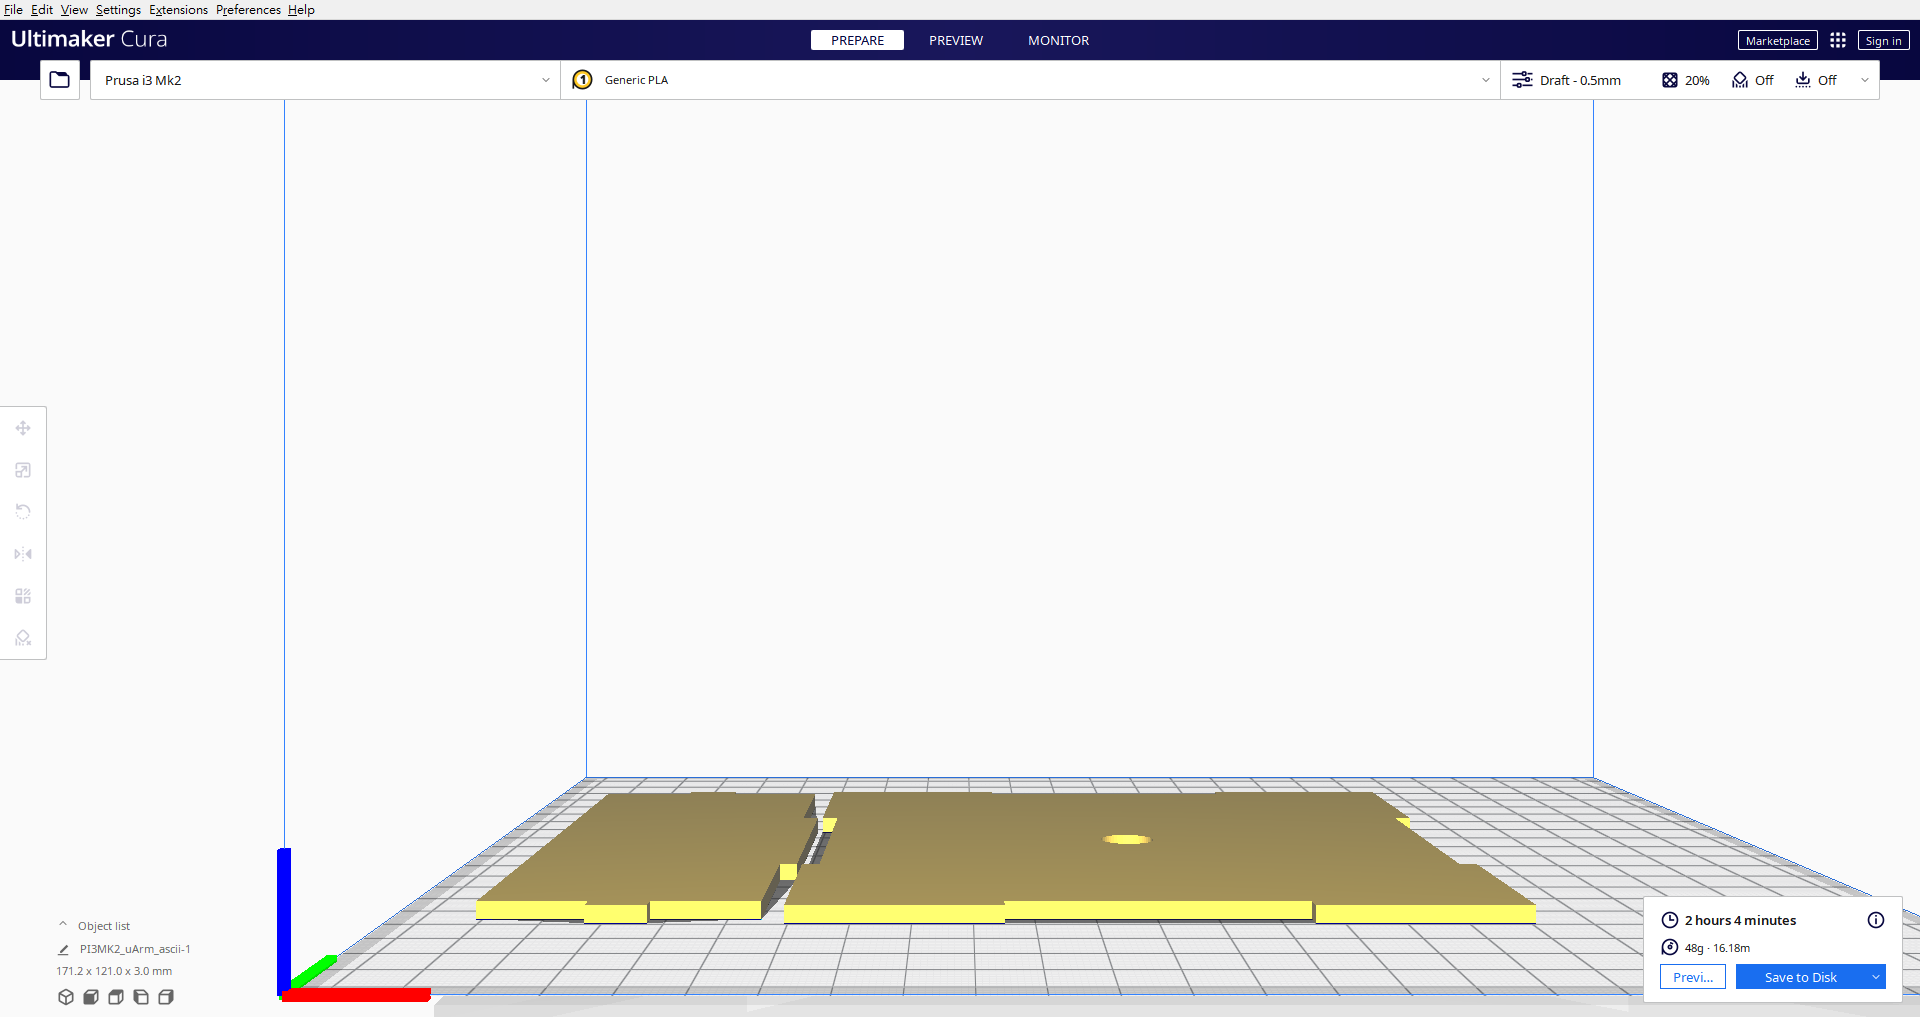
\includegraphics[width=14cm]{Cura}
\caption{\Large 用於轉出 G-Ccode 檔的切片軟體 Cura}\label{Cura}
\end{center}
\end{figure}
\section{更改G-Code檔}
 由於此列印模組之Z軸與本專題之3D列印機恰好相反,因此需修改有關的Z軸代碼後的數值為負值,還有一處需要修改,那就是擠出率的代碼,列印模組中擠出率代碼為A,但從Cura中轉出的G-Code中擠出率代碼為E,所以需將G-Code中的代碼E更改為A。
\begin{figure}[hbt!]
\begin{center}
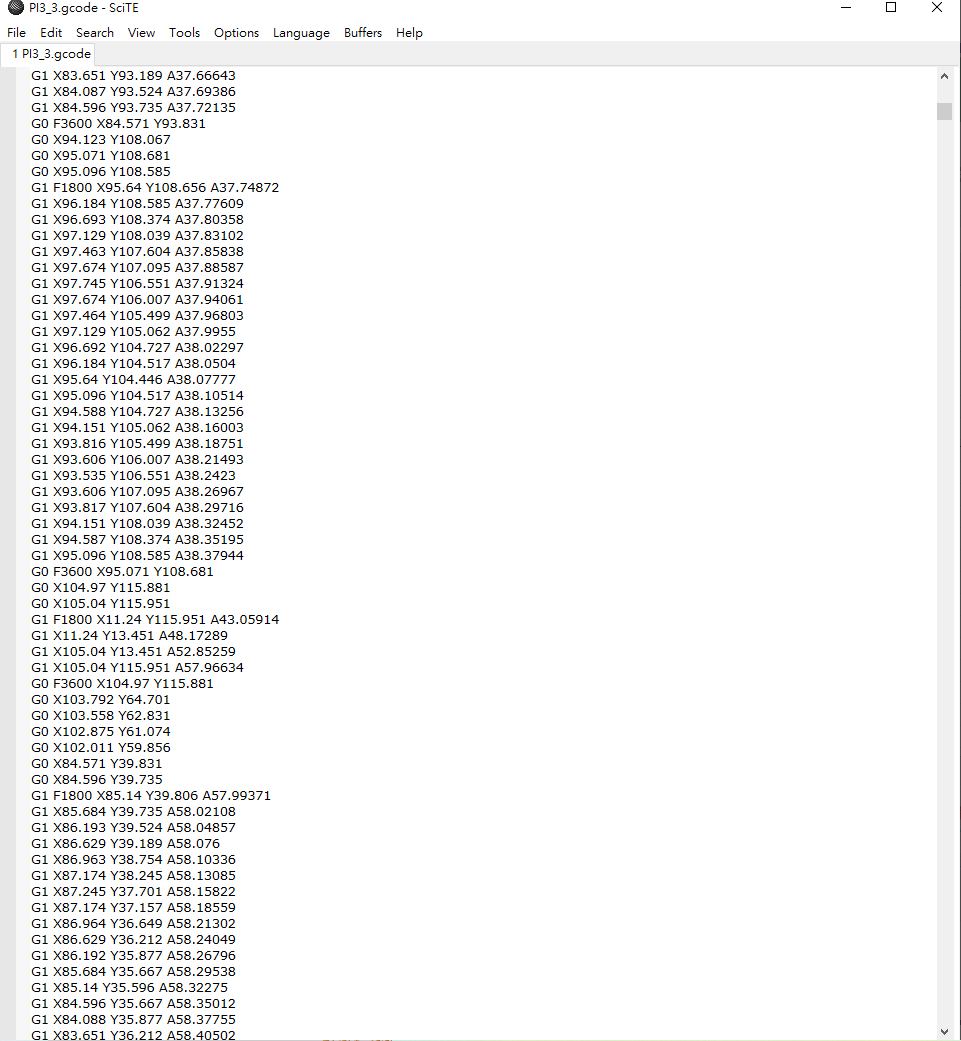
\includegraphics[width=14cm]{修改GCODE}
\caption{\Large 修改G-Code部分代碼}\label{修改GCODE}
\end{center}
\end{figure}
\section{將G-Code轉入GCodeInterpreter}
 第四步將修改好的G-Code檔案轉入GCodeInterpreter,按下連接鍵與CoppeliaSim連接後,進行模擬。\\
\begin{figure}[hbt!]
\begin{center}
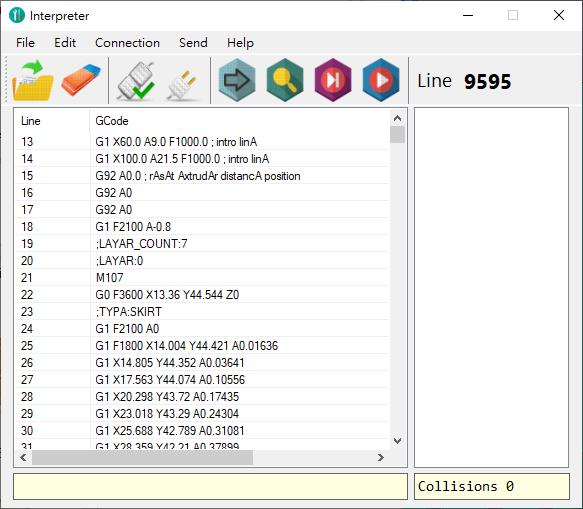
\includegraphics[width=14cm]{GCodeInterpreter}
\caption{\Large 模擬中的GCodeInterpreter畫面}\label{GCodeInterpreter}
\end{center}
\end{figure}
\section{uArm零件模擬列印結果}
 在CoppeliaSim模擬設定視窗中可以調整擠出材料的大小以及形狀(圓球或方塊),與GCodeInterpreter連接後,當GCodeInterpreter按下運行鍵後,開始列印模擬,在CoppeliaSim中也可以進行模擬列印整體速度調整,更加省時,下圖為模擬結果。\\
\begin{figure}[hbt!]
\begin{center}
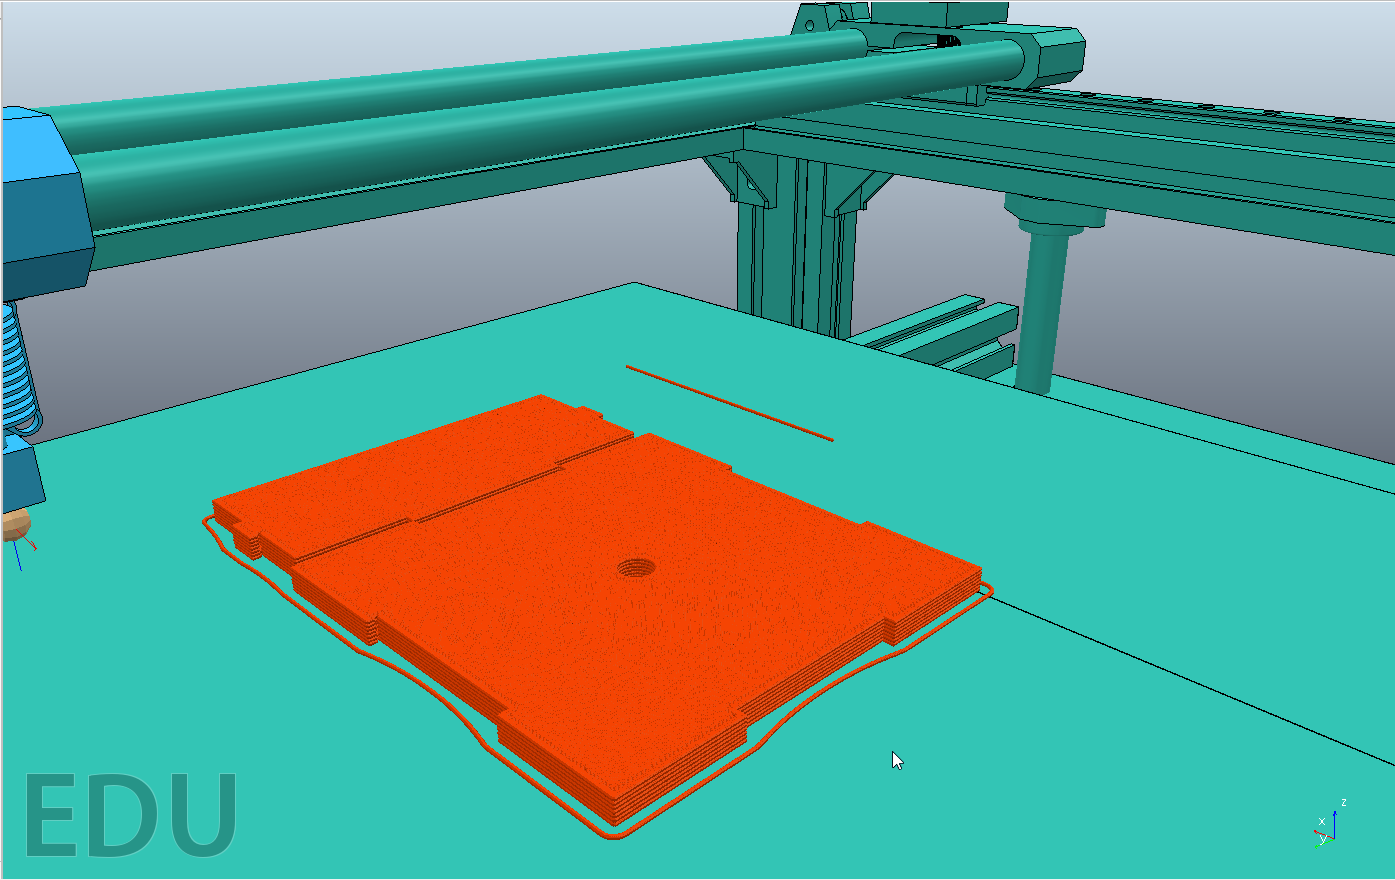
\includegraphics[width=14cm]{simulation}
\caption{\Large 模擬列印結果}\label{simulation}
\end{center}
\end{figure}

\begin{figure}[hbt!]
\begin{center}
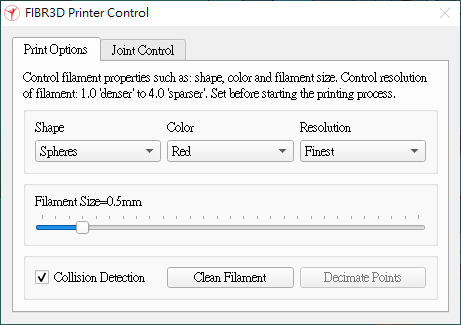
\includegraphics[width=12cm]{UIP}
\caption{\Large 列印選項控制 UI介面}\label{UIP}
\end{center}
\end{figure}

\section{在CoppeliaSim匯入uArm零件進行模擬}
 將uArm的STL檔可透過pySTL進行縮放後,匯入CoppeliaSim中將零件進行拆解並簡化,接著是各軸的組配,最後搭配CoppeliaSim的UI進行三個馬達軸的控制。\\
\subsection{簡化模型}
 所謂的簡化係指將uArm STL檔轉進CoppeliaSim拆解後,進入Toggle shape edit mode(三角形編輯模式)針對各零件的三角網格進行選擇後,從複雜形狀的零件簡化提取出方塊、圓柱或圓球等等的簡單形狀,用於模擬運算,外觀可套上原零件保持原樣,另一方式為使用add選單中的Convex decomposition of selection(凸分解),Convex Hull(凸包)可以理解在高維空間中有一群散佈各處的點,「凸包」是包覆這群點的所有外殼當中,表面積暨容積最小的一個外殼,而最小的外殼一定是凸的。而凸分解就是將零件依據三角網格的頂點分解成數個凸包再進行組合,在運算效率上來說使用Toggle shape edit mode(三角形編輯模式)方式可獲得較好的效果。\\
\begin{figure}[hbt!]
\begin{center}
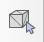
\includegraphics[width=2cm]{TSEM}
\caption{\Large Toggle shape edit mode(三角形編輯模式)}\label{TSEM}
\end{center}
\end{figure}

\begin{figure}[hbt!]
\begin{center}
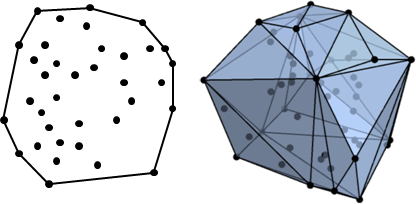
\includegraphics[width=10cm]{ConvexHull1}
\caption{\Large Convex Hull(凸包)}\label{ConvexHull1}
\end{center}
\end{figure}

\subsection{模擬}
 一開始使用官方圖檔進行模擬,花費許多組配時間在簡化零件之上,所以決定使用自行繪製的簡化圖檔進行模擬,簡化圖檔保留了主要的零件,設計後的零件大部分為利於列印的薄板件。\\
\begin{figure}[hbt!]
\begin{center}
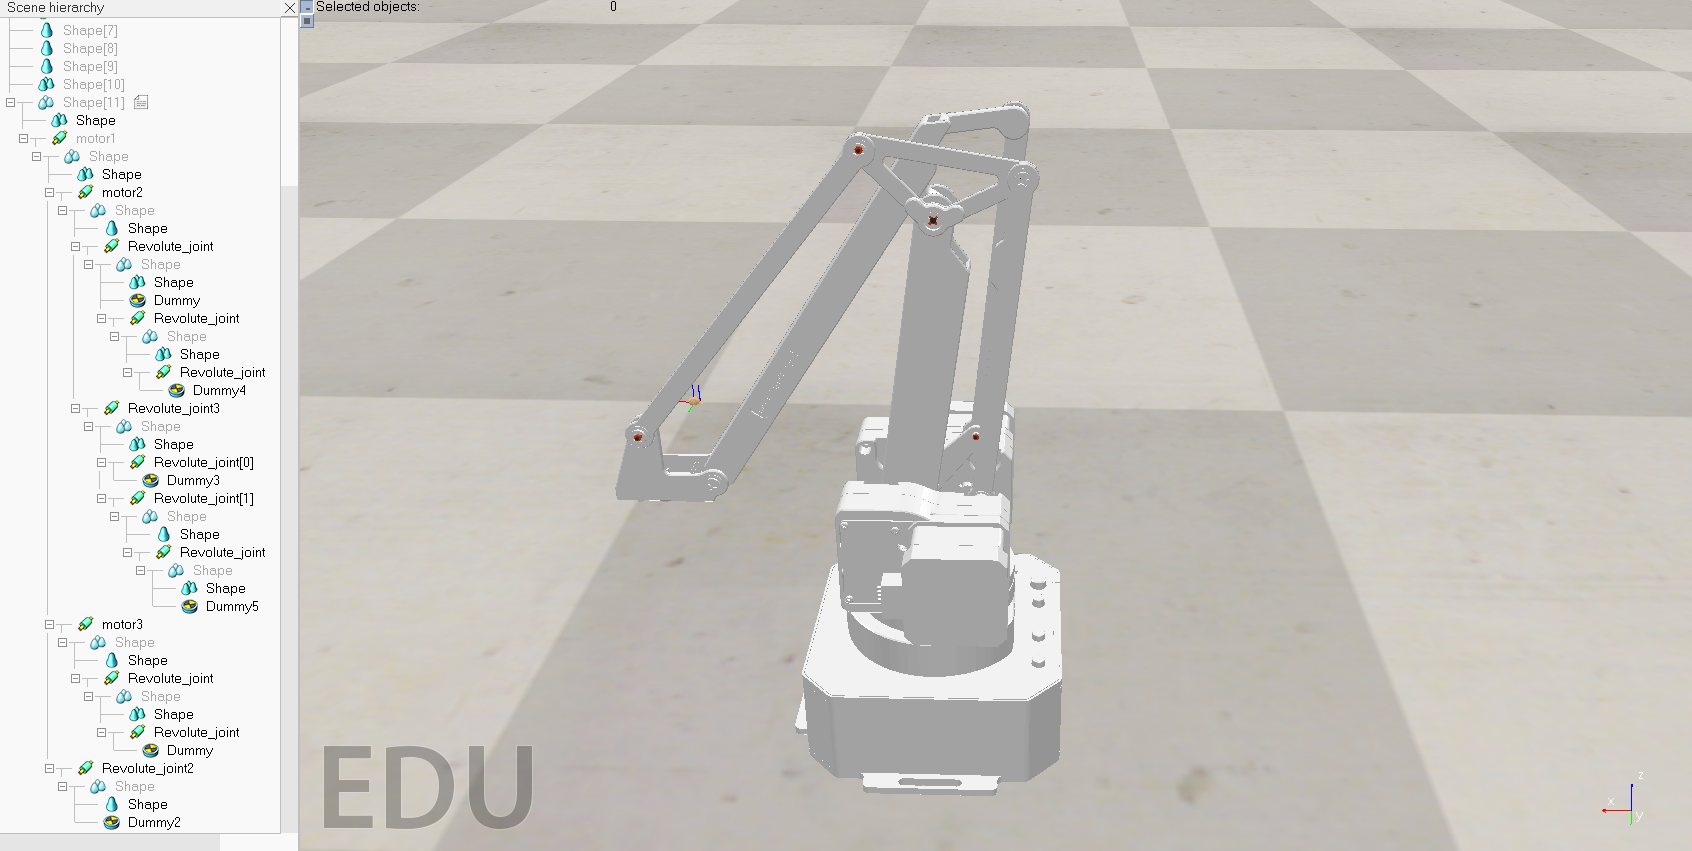
\includegraphics[width=14cm]{uArm01}
\caption{\Large 原版的uArm手臂模擬}\label{uArm01}
\end{center}
\end{figure}
\begin{figure}[hbt!]
\begin{center}
\includegraphics[width=14cm]{uArm02}
\caption{\Large 設計過後的uArm手臂模擬}\label{uArm02}
\end{center}
\end{figure}
\begin{figure}[hbt!]
\begin{center}
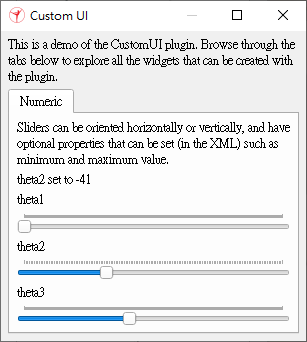
\includegraphics[width=12cm]{UI}
\caption{\Large 用於控制3個馬達軸的UI介面}\label{UI}
\end{center}
\end{figure}
\newpage

